\begin{center}
\textbf{
\MakeUppercase{Приложение А}\\
(обязательное)\\
Исходный код}
\end{center}
\addcontentsline{toc}{section}{Приложение А. Исходный код}

\lstinputlisting[style=js]{appendices/csharp/BotExtensions.cs}
\lstinputlisting[style=js]{appendices/csharp/CancelCommandHandlerService.cs}
\lstinputlisting[style=js]{appendices/csharp/CategoryCommandHandlerService.cs}
\lstinputlisting[style=js]{appendices/csharp/CommandService.cs}
\lstinputlisting[style=js]{appendices/csharp/DependencyInjectionExtensions.cs}
\lstinputlisting[style=js]{appendices/csharp/FinanceManagerBotController.cs}
\lstinputlisting[style=js]{appendices/csharp/GetMessage.cs}
\lstinputlisting[style=js]{appendices/csharp/HelpCommandHandlerService.cs}
\lstinputlisting[style=js]{appendices/csharp/StartCommandHandlerService.cs}
\lstinputlisting[style=js]{appendices/csharp/StatsService.cs}

\newpage
\begin{center}
\textbf{
\MakeUppercase{Приложение Б}\\
(Рекомендуемое)\\
Отчет сервиса антиплагиат}
\end{center}
\addcontentsline{toc}{section}{Приложение Б. Отчет сервиса антиплагиат}

\begin{figure}[!h]
	\centering
	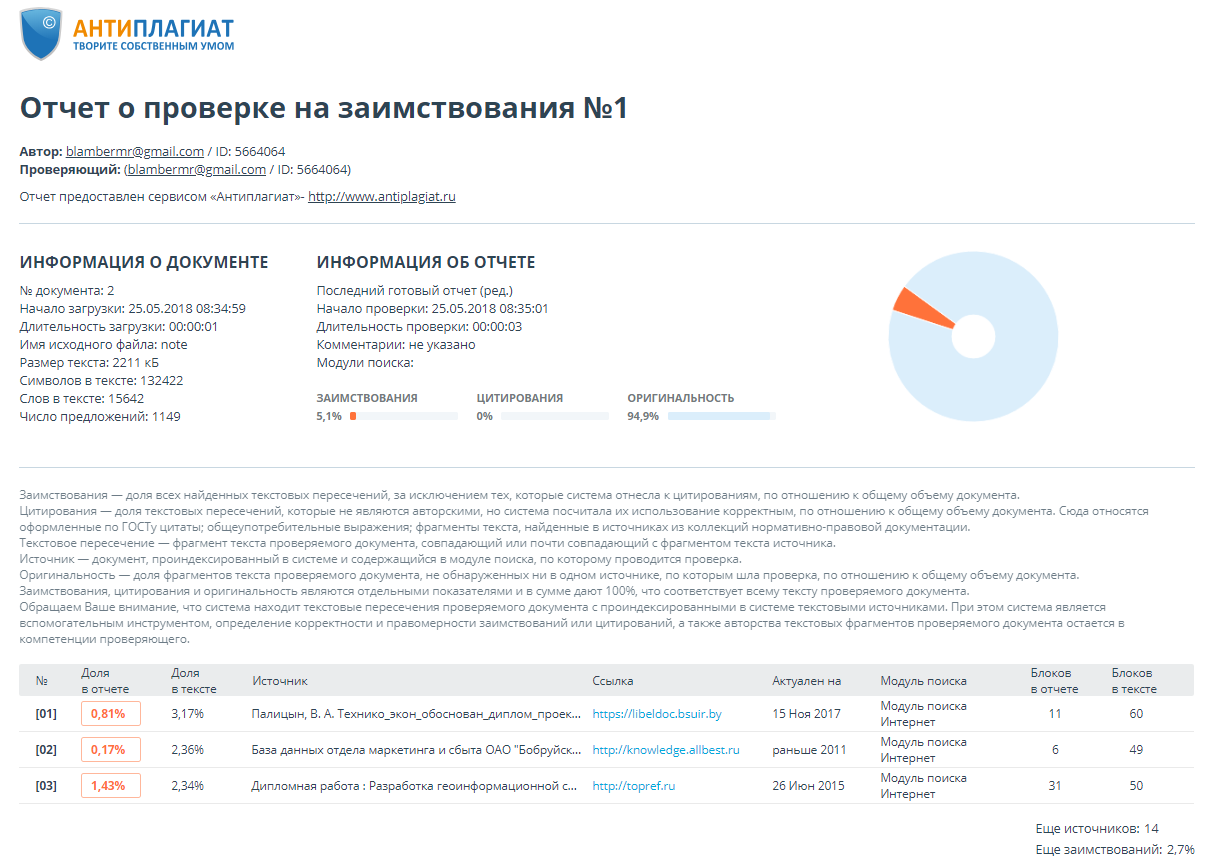
\includegraphics[scale=0.5]{antiplagiat.png} 
	\label{antiplagiat}
\end{figure}